\lecture[13]{Association \& Causation}{lecture-text}

\subtitle{and statistical significance}

\date{14 October 2015}


\begin{document}

\begin{frame}
  \maketitle
\end{frame}

\begin{frame}{Last time}

    \begin{itemize}
        \item Errors are of two types: 
            \begin{itemize}
                \item[(I)] \alert{no} real difference, but we are misled by noise
                \item[(II)] \alert{real} difference, but we can't tell, because of noise
            \end{itemize}
        \item \structure{Significance level} is a false positive rate 
        \item \structure{Statistical power} is the probability of finding a real pattern.
        \item Doing an \alert{one-sided} test can increase your power.
    \end{itemize}

\end{frame}

\section*{Introduction}
\begin{frame}\frametitle<presentation>{Outline}
  \begin{quote}
    ``The statistical analysis should aid the researcher by helping to clarify whatever
    message is contained in the data.''
  \end{quote}
  \tableofcontents
\end{frame}


\section{Association and Causation}

\begin{frame}{What happens in a study}

    \alert{Question:} Does $X$ affect $Y$?

    \vspace{2em}

    To find out, we take some samples, recording:
      \begin{enumerate}
          \item explanatory variable(s) ($X$)
          \item response variable(s) ($Y$)
      \end{enumerate}
    and the typical value of $Y$ seems to depend on $X$.

    \vspace{2em}

    \ldots but then, what do we conclude?

    \vspace{2em}

    \alert{It depends} on how we take the sample.

\end{frame}

\begin{frame}{Example: hematocrit}

    \alert{Hematocrit} measures concentration of red blood cells in blood.
    Are sex differences caused by androstenedione?

    \vspace{2em}

    \only<1>{
    \begin{block}{Males \& Females}
        From sample of 489 males and 469 females:

        \vspace{1em}

        \centering
        \begin{tabular}{l|rr}
            & Males & Females \\
            \hline
            Mean & 45.8 & 40.6 \\
            SD & 2.8 & 2.9 \\
        \end{tabular}
    \end{block}
    }

    \only<2>{
    \begin{block}{High \& low hormone levels}
        From sample of 489 ``low'' and 469 ``high'' 
        levels of androstenedione:

        \vspace{1em}

        \centering
        \begin{tabular}{l|rr}
            & Low & High \\
            \hline
            Mean & 45.8 & 40.6 \\
            SD & 2.8 & 2.9 \\
        \end{tabular}

        \tiny (fake data)
    \end{block}
    }

    \only<3>{
    \begin{block}{Controlled hormone levels}
        From sample of 489 males and 469 females,
        random set of half of each had
        artificially induced levels of androstenedione:

        \vspace{1em}

        \centering
        \begin{tabular}{l|rr}
            & Low & High \\
            \hline
            Mean & 45.8 & 40.6 \\
            SD & 2.8 & 2.9 \\
        \end{tabular}

        \tiny (fake data)
    \end{block}
    }


    \vspace{2em}

    What do we conclude?

\end{frame}

%%%%%
\subsection{Experimental vs.\ Observational studies}

\begin{frame}{There's more to an experiment than observation.}

  \begin{block}{How to do an observational study}
    \alert{Observe} (measure) something about an existing situation.
  \end{block}

  \vspace{2em}

  \begin{block}{How to do an experimental study}
    Observe (measure) something
    from groups whose \structure{differences} were \alert{chosen} by you.
  \end{block}

  \vspace{2em}

  \alert{Easy way to get experimental:}
  Randomly assign to treatment and control groups.

  \vspace{2em}

  \begin{quote}
    In an \textbf{experiment}, the researcher manipulates the experimental conditions,
    \textbf{defining} the populations being compared.
  \end{quote}

\end{frame}

%
\begin{frame}{Observation versus experiment}

  Is it an observational study or an experimental study?
  \begin{enumerate}

    \item How were the samples obtained?

    \item Who is in the treatment and the control groups? \\
      \alert{or} Does the researcher assign the explanatory variables?

    \item Who is being studied?

  \end{enumerate}

  \vspace{2em}

  \begin{quote}
    In an \textbf{experiment}, the researcher manipulates the experimental conditions,
    \textbf{defining} the populations being compared.
  \end{quote}

\end{frame}

%
\begin{frame}{}


  {\small
  ``\emph{Physical activity, fitness, glucose homeostasis, and brain morphology in twins.}'', 
  \url{http://www.ncbi.nlm.nih.gov/pubmed/25003773}
  }
  \begin{center}
    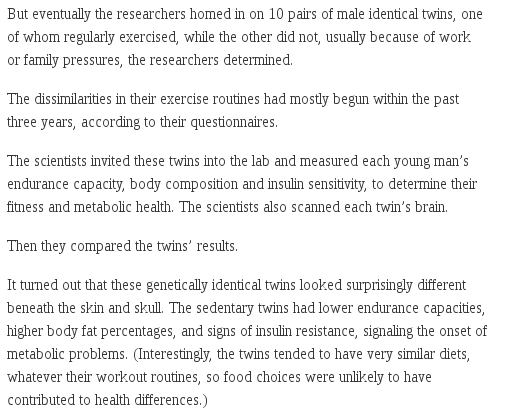
\includegraphics[width=0.85\textwidth]{examples/twins-exercise_news}
  \end{center}
  \flushright\small\figcaption{\url{http://well.blogs.nytimes.com/2015/03/04/one-twin-exercises-the-other-doesnt}}


\end{frame}

%
\begin{frame}{The difference}

  In \alert{both} observational and experimental studies,
  the conclusion is generally ``$X$ is associated with $Y$'' (or not).

  \vspace{2em}

  \ldots but in an \alert{experiment},
  there are a lot fewer ways to explain the association.

  \vspace{2em}

  \structure{Example:}
  \begin{description}
      \item[Study 1:] Children of smokers have lower birth weight.
        \pause
      \item[Study 2:] We got a randomly chosen half of our sample to start smoking,
          and their children had lower birth weight.
  \end{description}

\end{frame}


%%%
\subsection{Correlation is not causation}

%
\begin{frame}{Correlation is not Causation}

  \begin{center}
  \includegraphicscopyright[width=6cm]{xkcd-correlation}{xkcd.com/552}

  \figcaption{``Correlation doesn't imply causation, but it does waggle its eyebrows suggestively and gesture furtively while mouthing `look over there'.''}
  \end{center}

  \vspace{2em}

  \alert{Why not?}

\end{frame}

%%%
\subsection{Confounding factors}

%
\begin{frame}{Confounding factors}

If we are looking for the effect of $X$ on $Y$,
the factor $Z$ is \alert{confounding} if $Z$ is known to have an effect on $Y$,
and $X$ might be associated with $Z$.

\vspace{2em}

If association between $X$ and $Y$ only happens because of $Z$:
\[
  X \sim Z \longrightarrow Y
\]
then the association is \alert{spurious}.

\vspace{2em}

\alert{Solution:} control for $Z$.  (can be difficult)

\vspace{2em}

\structure{Study 2':} We got 159 pairs of women,
    each matching in many ways, except one of the pair quit smoking before the second pregnancy.
    Those who quit had heavier children.

\end{frame}

\begin{frame}{Exercise}

  \begin{center}
  \includegraphicscopyright[width=.9\textwidth]{ss-7-4-5}{Samuels, Whitmer, \& Schaffner}
  \end{center}


\end{frame}


%%%%%% %%%%%%
\section{Significant or important?}

\subsection{Unpacking the terminology}


%%%%%%
\begin{frame}{Interpreting results}

  % \begin{quote}
  %   \textbf{Results:}
  %   According to pairwise analysis, the active twins had lower body fat percentage ($P=0.029$) and homeostatic model assessment index ($P=0.031$) and higher Matsuda index ($P=0.021$) compared with their inactive co-twins.  Striatal andprefrontal cortex (subgyral and inferior frongal gyrus) brain gray matter volumes were larger in the nondominant hemisphere in active twins compared with those in inactive co-twins, with a statistical threshold of $P<0.001$.
  % \end{quote}
  \begin{center}
    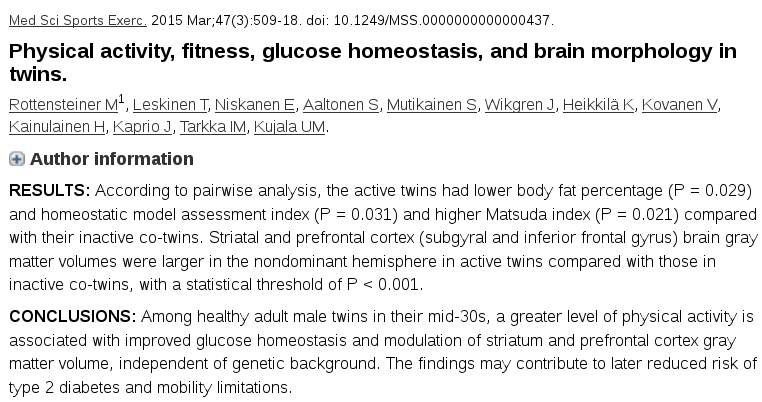
\includegraphics[width=\textwidth]{examples/twins-exercise_abstract_results}
  \end{center}
  \flushright{\small \url{http://www.ncbi.nlm.nih.gov/pubmed/25003773}}

  \vspace{2em}

  Let's unpack those statements.

\end{frame}

%%%%%%
\begin{frame}{Statistical significance}

    \begin{quote}
        had \only<2->{\alert{statistically significantly} }lower body fat percentage ($P=0.029$),
        \only<3->{\alert{at the $\alpha=0.05$ significance level}}
    \end{quote}

    \uncover<4->{
    \structure{means, roughly}
    \begin{quote}
        we found good evidence that the differences was not caused by chance variation alone
    \end{quote}
    }

    \uncover<5->{
    \structure{or more precisely}
    \begin{quote}
        if the null hypothesis was true, we'd expect to see at least this large a difference no more than 5\% of the time
    \end{quote}
    }

\end{frame}

%%%%%%
\begin{frame}{Lack of statistical signficance}

    \begin{quote}
      no \only<2->{\alert{statistically significant }}difference was found in body mass index ($P=0.28$) \only<2->{\alert{at the $\alpha=0.05$ signficance level}}
    \end{quote}

    \uncover<3->{
    \structure{means, roughly}
    \begin{quote}
        there was not sufficient evidence that the observed difference was due to anything other than chance variation
    \end{quote}
    }

    \uncover<3->{
    \structure{or more precisely}
    \begin{quote}
        if the null hypothesis was true, we'd expect to see at least this large a difference \alert{at least} 5\% of the time
    \end{quote}
    }

\end{frame}

%%%%%%
\begin{frame}{Example}

  Lactate dehydrogenase levels:
  \begin{center}
    \begin{tabular}{crr}
       & Males & Females \\
       \hline
       $n$ & 270 & 264 \\
       $\bar y$ & 60 & 57 \\
       $s$ & 11 & 10
     \end{tabular}

   \vspace{2em}

   \uncover<2->{$t_s=3.3$ and $P=0.001$}
   \end{center}

\end{frame}


%%%%%%
\begin{frame}{Example}

  Body weight:
  \begin{center}
    \begin{tabular}{crr}
       & Males & Females \\
       \hline
       $n$ & 2 & 2 \\
       $\bar y$ & 175 & 143 \\
       $s$ & 35 & 34
     \end{tabular}

   \vspace{2em}

   \uncover<2->{$t_s=0.93$ and $P=0.45$}
   \end{center}

\end{frame}


%%%%%%
\begin{frame}{Interpret:}

    \begin{quote}
        The subjects were given varying doses of the drug and also a placebo in a double-blind randomized trial. Researchers found low doses [...] improved memory performance[.]
    \end{quote}
    \figcaption{\textit{Drug restores brain function and memory in early Alzheimer's disease}, \url{http://www.sciencedaily.com/releases/2015/03/150311124200.htm}}

    \vfill
    \pause

    \begin{quote}
        We observed significant improvement in memory task performance under drug treatment relative to placebo in the aMCI cohorts at the 62.5 and 125 mg BID doses of levetiracetam.
    \end{quote}
    \figcaption{\url{http://www.sciencedirect.com/science/article/pii/S2213158215000273}}

\end{frame}



%%%%%% %%%%%% %%%%%% %%%%%%
\section{Describing real-world importance}

%%%%%%%
\begin{frame}{Significant or important?}
    \vfill

    So you have a \alert{tiny $P$-value}.

    \vfill

    How big is the effect?

    \vfill
    \pause

    \structure{Or,} I believe your result is not noise,
    but how much \alert{do I care?}

\end{frame}

%%%%%%
\begin{frame}{It's significant, but is it important?}


    \begin{block}{the difference in means}
        We've observed a difference between two populations:
        \[  \bar y_1 - \bar y_2 \]
    \end{block}

    \ldots and got a small $P$-value.  So what?

    \vspace{2em}

    \structure{Ask yourself:} What do we want to know?\\

    \vspace{2em}

    How important is the observed difference?


\end{frame}


%%%%%% %%%%%%
\subsection{The effect size}

%%%%%%
\begin{frame}{}

    \begin{block}<1->{the $t$-statistic}
        \begin{align*}
            t_s = \frac{\bar y_1 - \bar y_2}{ \SE_{\bar Y_1 - \bar Y_2} } 
            = \frac{ \text{(actual difference)} }{ \text{(magnitude of sampling noise)} }
        \end{align*}
        is big if the observed difference is large compared to the estimated size of the \alert{estimation error}.
    \end{block}

    \begin{block}<2->{the effect size}
        If both populations have the same SD, $\sigma$,
        \begin{align*}
            \text{(Effect size)} = \frac{\bar y_1 - \bar y_2}{ \sigma }
            = \frac{ \text{(actual difference)} }{ \text{(magnitude of within-population variation)} }
        \end{align*}
        is big if the observed difference is large compared to \alert{within-population variation}.
    \end{block}

\end{frame}

%%%%%%
\begin{frame}{Examples}
    In each, 
    what are the $t$-statistics
    and the effect sizes?
    What do they tell us?

  \vfill

  Lactate dehydrogenase levels:
  \begin{center}
    \begin{tabular}{crr}
       & Males & Females \\
       \hline
       $n$ & 270 & 264 \\
       $\bar y$ & 60 & 57 \\
       $s$ & 11 & 10
     \end{tabular}
  \end{center}
  
  \vfill

  Body weight (lb):
  \begin{center}
    \begin{tabular}{crr}
       & Males & Females \\
       \hline
       $n$ & 2 & 2 \\
       $\bar y$ & 175 & 143 \\
       $s$ & 35 & 34
     \end{tabular}
 \end{center}

\end{frame}


%%%%%% %%%%%%
\subsection{Using confidence intervals}

%%%%%%
\begin{frame}{Significantly unimportant?}

    The \alert{confidence interval} describes where we are pretty confident the true value lies.

    \begin{itemize}

    \item So if we think an effect smaller than $x$ is \alert{unimportant}
      and $x$ is outside the confidence interval,

    \item then we have good evidence the true effect is unimportant.
      (inconsequential, insignificant, \ldots?)

    \end{itemize}

    \vspace{2em}

    Examples:
    \begin{itemize}
      \item Lactate dehydrogenase levels:
      \item Body weight:
    \end{itemize}

\end{frame}

%%%%%%
\begin{frame}{Interpret:}

  \begin{quote}
    ``Our data also suggest a positive association of cigarette smoking and new HPV detection (OR, 3.4; 95\% CI, 0.4--26.3); {however, because 87\% of study participants were smokers, we had limited power to detect significant effects.}''
  \end{quote}

  \vspace{2em}

  OR = ``odds ratio'' = increased odds of contracting HPV

\end{frame}


%%%%%%
\begin{frame}{Not significant, but important?}

    Recall that ``not signficant'' means
    \begin{quote}
        there was not sufficient evidence that the observed difference was due to anything other than chance variation.
    \end{quote}


    \vspace{2em}

    This does \alert{not} mean that there is no real difference!

    \vspace{2em}

    If the confidence interval includes zero, but also some big (important) values,
    then we don't have the \alert{power} to tell.  
    Here ``not significant'' reflects our uncertainty.



\end{frame}


%%%%%%
\begin{frame}{Tomato yield}

    Comparing the yield of two tomato varieties,
    a mean difference of 1 pound per plant is ``important''.

    \vspace{2em}

    \begin{center}
    \begin{tabular}{c|cc}
        95\% CI & significant? & important? \\
        \hline
        0.2 -- 0.3 & & \\
        1.2 -- 1.3 & & \\
        0.2 -- 1.3 & & \\
        -0.2 -- 0.3 & & \\
        -1.2 -- 0.3 & & \\
        \hline
    \end{tabular}
    \end{center}


\end{frame}


%%%%%%
\mode<presentation>{
\begin{frame}{Tomato yield}

    Comparing the yield of two tomato varieties,
    a mean difference of 1 pound per plant is ``important''.

    \vspace{2em}

    \begin{center}
    \begin{tabular}{c|cc}
        95\% CI & significant? & important? \\
        \hline
        0.2 -- 0.3 & yes & no \\
        1.2 -- 1.3 & yes & yes \\
        0.2 -- 1.3 & yes & don't know \\
        -0.2 -- 0.3 & no & no \\
        -1.2 -- 0.3 & no & don't know \\
        \hline
    \end{tabular}
    \end{center}


\end{frame}
}


%
\begin{frame}{What's missing?}
  \begin{center}
    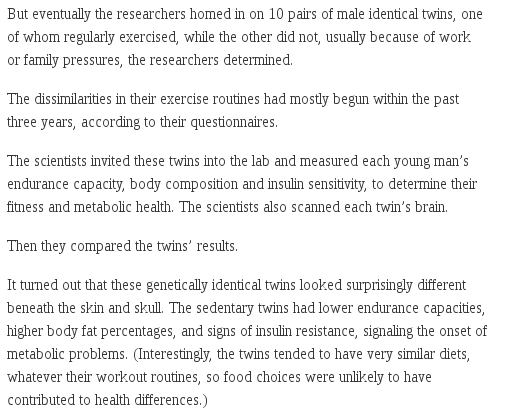
\includegraphics[width=0.85\textwidth]{examples/twins-exercise_news}
  \end{center}
  \flushright\small\figcaption{\url{http://well.blogs.nytimes.com/2015/03/04/one-twin-exercises-the-other-doesnt}}
\end{frame}

%
\begin{frame}{Is it here?}
  {\small
  ``{Physical activity, fitness, glucose homeostasis, and brain morphology in twins.}'', 
  }
  \begin{center}
    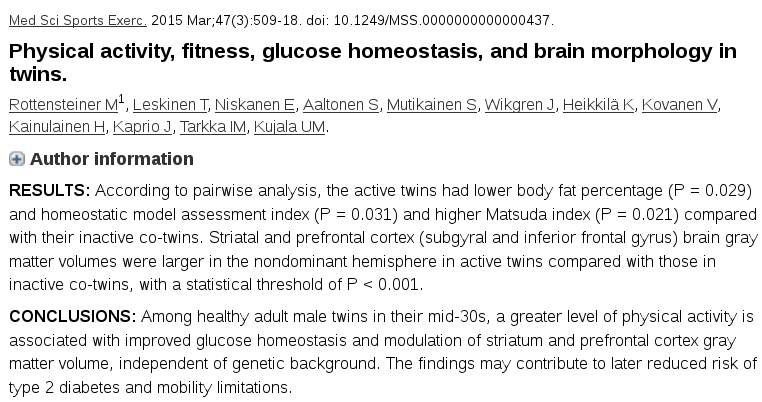
\includegraphics[width=\textwidth]{examples/twins-exercise_abstract_results}
  \end{center}
  \flushright\small\figcaption{
  ``Physical activity, fitness, glucose homeostasis, and brain morphology in twins.'', 
  \url{http://www.ncbi.nlm.nih.gov/pubmed/25003773}
  }
\end{frame}

%
\begin{frame}[plain]{The results}
  \begin{center}
    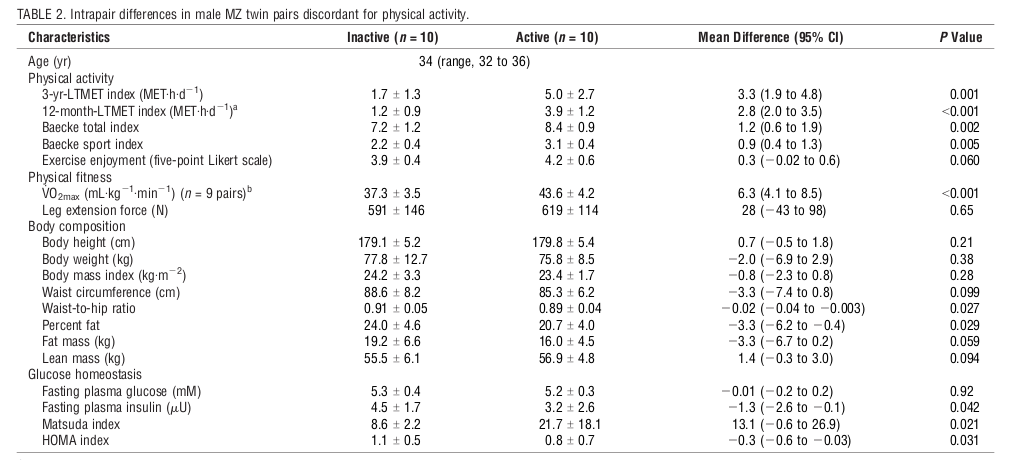
\includegraphics[width=1.2\textwidth]{examples/twins-exercise_study-results}
  \end{center}
  \flushright\small\figcaption{
  \url{http://www.ncbi.nlm.nih.gov/pubmed/25003773}
  }
\end{frame}


%%%%%
\section<article>{Summary}
\section<presentation>*{Summary}

\begin{frame}{Summary}

  \begin{itemize}
    \item An \alert{observational study} observes an existing situation,
    \item to look for correlations.
    \item But, \alert{correlation is not causation},
    \item thanks in part to \alert{confounding factors}.
    \item \alert{Experimental studies} try to eliminate these,
    \item so provide much stronger evidence of causation.
  \end{itemize}

    \vspace{1em}

    \begin{itemize}
        \item Statistical signficance \alert{does not imply} \\real--world significance.
        \item Lack of statistical signficance \alert{does not imply} \\real--world insignificance.
        \item Sample size acts like a \structure{magnifying glass}, making smaller differences visible.
        \item The \alert{effect size} describes the scale of a difference.
        \item Confidence intervals communicate both statistical signficance and real--world importance.
    \end{itemize}
\end{frame}

% homework
\begin{frame}{Homework}

  \begin{center}

    7.4.6

  \vspace{2em}

    7.6.1

  \vspace{2em}

  Email me an interesting scientific study reported on in the news.

  \end{center}

\end{frame}



\end{document}





